\part{Logic gates}
\frame{\partpage}

\newcommand{\TT}{\textsc{True}}
\newcommand{\FF}{\textsc{False}}
\newcommand{\OP}[1]{\ \textsc{#1}\ }
\newcommand{\OPand}{\OP{and}}
\newcommand{\OPor}{\OP{or}}
\newcommand{\OPxor}{\OP{xor}}
\newcommand{\OPnand}{\OP{nand}}
\newcommand{\OPnor}{\OP{nor}}
\newcommand{\OPxnor}{\OP{xnor}}
\newcommand{\OPnot}{\textsc{not}\ }

\newcommand{\OPname}{}
\newcommand{\OPenglishA}{}
\newcommand{\OPenglishB}{}
\newcommand{\OPtable}{}
\newcommand{\OPdiagram}{}

\newcommand{\OPframe}[5]{
	\begin{frame}{#1}
		\pause
		\begin{center}
			#2 \par if and only if \par #3
		\end{center}
		\pause
		\begin{columns}
			\begin{column}{0.48\textwidth}
				\begin{center}
					#4
				\end{center}
			\end{column}
			\pause
			\begin{column}{0.48\textwidth}
				\begin{center}
					\begin{circuitikz} \draw[color=\circuitcolour]
						#5
					\end{circuitikz}
				\end{center}
			\end{column}
		\end{columns}
	\end{frame}
}

\begin{frame}{Boolean logic}
	\begin{itemize}
		\pause\item Works with two values: \TT\ and \FF
		\pause\item Foundation of the \textbf{digital computer}:
			represented in circuits as \textbf{on} and \textbf{off}
		\pause\item Representing as $1$ and $0$ leads to \textbf{binary notation}
		\pause\item One boolean value = one \textbf{bit} of information
		\pause\item Programmers use boolean logic for conditions in \lstinline{if} and \lstinline{while}
			statements
	\end{itemize}
\end{frame}

%\begin{frame}{Simulating logic circuits}
	%\centering
	%\url{http://logic.ly/demo/}
%\end{frame}

\OPframe{Not}
	{$\OPnot A$ is \TT}{$A$ is \FF}
	{\begin{tabular}{|c||c|} \hline
		$A$ & $\OPnot A$ \\\hline
		\FF & \TT \\
		\TT & \FF \\\hline
	\end{tabular}}
	{ (0,0) node[not port] (gate) {}
	(gate.in)  node[anchor=east] {$A$}
	(gate.out) node[anchor=west] {$\OPnot A$}
	; }

\OPframe{And}
	{$A \OPand B$ is \TT}{\textbf{both $A$ and $B$} are \TT}
	{\begin{tabular}{|c|c||c|}
		\hline
		$A$ & $B$ & $A \OPand B$ \\\hline
		\FF & \FF & \FF \\
		\FF & \TT & \FF \\
		\TT & \FF & \FF \\
		\TT & \TT & \TT \\\hline
	\end{tabular}}
	{ (0,0) node[and port] (gate) {}
	(gate.in 1) node[anchor=east] {$A$}
	(gate.in 2) node[anchor=east] {$B$}
	(gate.out)  node[anchor=west] {$A \OPand B$}
	; }

\OPframe{Or}
	{$A \OPor B$ is \TT}{\textbf{either $A$ or $B$, or both,} are \TT}
	{\begin{tabular}{|c|c||c|}
		\hline
		$A$ & $B$ & $A \OPand B$ \\\hline
		\FF & \FF & \FF \\
		\FF & \TT & \TT \\
		\TT & \FF & \TT \\
		\TT & \TT & \TT \\\hline
	\end{tabular}}
	{ (0,0) node[or port] (gate) {}
	(gate.in 1) node[anchor=east] {$A$}
	(gate.in 2) node[anchor=east] {$B$}
	(gate.out)  node[anchor=west] {$A \OPor B$}
	; }

\begin{frame}{Socrative \texttt{FALCOMPED}}
	What is the value of
	$$ A \OPand (B \OPor C) $$
	when
	\begin{align*}
		A &= \TT \\
		B &= \FF \\
		C &= \TT
	\end{align*}
	?
\end{frame}

\begin{frame}{Socrative \texttt{FALCOMPED}}
	What is the value of
	$$ (\OPnot A) \OPand (B \OPor C) $$
	when
	\begin{align*}
		A &= \TT \\
		B &= \FF \\
		C &= \TT
	\end{align*}
	?
\end{frame}

\begin{frame}{Socrative \texttt{FALCOMPED}}
	For what values of $A, B, C, D$ is
	$$ A \OPand \OPnot B \OPand \OPnot (C \OPor D) = \TT $$
	?
\end{frame}

\begin{frame}{Socrative \texttt{FALCOMPED}}
	What is the value of
	$$ A \OPor \OPnot A $$
	?
\end{frame}

\begin{frame}{Socrative \texttt{FALCOMPED}}
	What is the value of
	$$ A \OPand \OPnot A $$
	?
\end{frame}

\begin{frame}{Socrative \texttt{FALCOMPED}}
	What is the value of
	$$ A \OPor A $$
	?
\end{frame}

\begin{frame}{Socrative \texttt{FALCOMPED}}
	What is the value of
	$$ A \OPand A $$
	?
\end{frame}

\begin{frame}{Socrative \texttt{FALCOMPED}}
	What expression is equivalent to this circuit?
	\begin{center}
		\begin{circuitikz} \draw[color=\circuitcolour]
			(0,0) node[and port] (gateA) {}
			(0,-2) node[or port] (gateB) {}
			(1,0) node[not port] (gateC) {}
			(3.5,-1) node[or port] (gateD) {}
			(gateA.out) -- (gateC.in) {}
			(gateC.out) -| (gateD.in 1) {}
			(gateB.out) -| (gateD.in 2) {}
			(gateD.out) node[anchor=west] {?}
			(gateA.in 1) node[anchor=east] {$A$}
			(gateA.in 2) node[anchor=east] {$B$}
			(gateB.in 1) node[anchor=east] {$C$}
			(gateB.in 2) node[anchor=east] {$D$}
			;
		\end{circuitikz}
	\end{center}
\end{frame}

\begin{frame}[fragile]{Writing logical operations}
	\pause
	\centering
	\begin{tabular}{|c||c|c|c|}
		\hline
		Operation & Python & C family & Mathematics \\\hline
		$\OPnot A$
			& \texttt{not a}
			& \texttt{!a}
			& $\neg A$ {\huge\phantom{$I$}} or {\huge\phantom{$I$}} $\overline{A}$
			\pause\\
		$A \OPand B$ 
			& \texttt{a and b}
			& \texttt{a \&\& b}
			& $A \wedge B$
			\pause\\
		$A \OPor B$ 
			& \texttt{a or b}
			& \texttt{a || b}
			& $A \vee B$
			\\\hline
	\end{tabular}
	\pause
	\par\vspace{2ex}\par
	Other operators can be expressed by combining these
\end{frame}

\begin{frame}{De Morgan's Laws}
	\pause
	$$ \OPnot (A \OPor B) = (\OPnot A) \OPand (\OPnot B) $$
	\pause
	$$ \OPnot (A \OPand B) = (\OPnot A) \OPor (\OPnot B) $$
	\pause
	Proof: Worksheet 4, questions 3a and 3b
\end{frame}

\part{Truth tables}
\frame{\partpage}

\begin{frame}{Enumeration}
	\begin{itemize}
		\pause\item Since booleans have only two possible values, we can often \textbf{enumerate}
			all possible values of a set of boolean variables
		\pause\item For $n$ variables there are $2^n$ possible combinations
		\pause\item Essentially, all the $n$-bit binary numbers
		\pause\item A \textbf{truth table} enumerates all the possible values of a boolean expression
		\pause\item Can be used to prove that two expressions are equivalent
	\end{itemize}
\end{frame}

\begin{frame}{Truth table example}
	$$ (A \OPor \OPnot B) \OPand C $$
	\begin{centering}
	    \small
		\begin{tabular}{|ccc|cc|c|}
		    \hline
			$A$ & $B$ & $C$ & $\OPnot B$ & $A \OPor \OPnot B$ & $(A \OPor \OPnot B) \OPand C$ \\\hline\pause
			\FF & \FF & \FF & \TT & \TT & \FF \\\pause
			\FF & \FF & \TT & \TT & \TT & \TT \\\pause
			\FF & \TT & \FF & \FF & \FF & \FF \\\pause
			\FF & \TT & \TT & \FF & \FF & \FF \\\pause
			\TT & \FF & \FF & \TT & \TT & \FF \\\pause
			\TT & \FF & \TT & \TT & \TT & \TT \\\pause
			\TT & \TT & \FF & \FF & \TT & \FF \\\pause
			\TT & \TT & \TT & \FF & \TT & \TT \\\hline
		\end{tabular}
	\end{centering}
\end{frame}

\part{Other logic gates}
\frame{\partpage}

\OPframe{Exclusive Or}
	{$A \OPxor B$ is \TT}{\textbf{either $A$ or $B$, but not both,} are \TT}
	{\begin{tabular}{|c|c||c|}
		\hline
		$A$ & $B$ & $A \OPand B$ \\\hline
		\FF & \FF & \FF \\
		\FF & \TT & \TT \\
		\TT & \FF & \TT \\
		\TT & \TT & \FF \\\hline
	\end{tabular}}
	{ (0,0) node[xor port] (gate) {}
	(gate.in 1) node[anchor=east] {$A$}
	(gate.in 2) node[anchor=east] {$B$}
	(gate.out)  node[anchor=west] {$A \OPxor B$}
	; }

\begin{frame}{Socrative \texttt{FALCOMPED}}
	How can $A \OPxor B$ be written using the operations $\OPand, \OPor, \OPnot$?
\end{frame}

\begin{frame}
    \begin{center}
        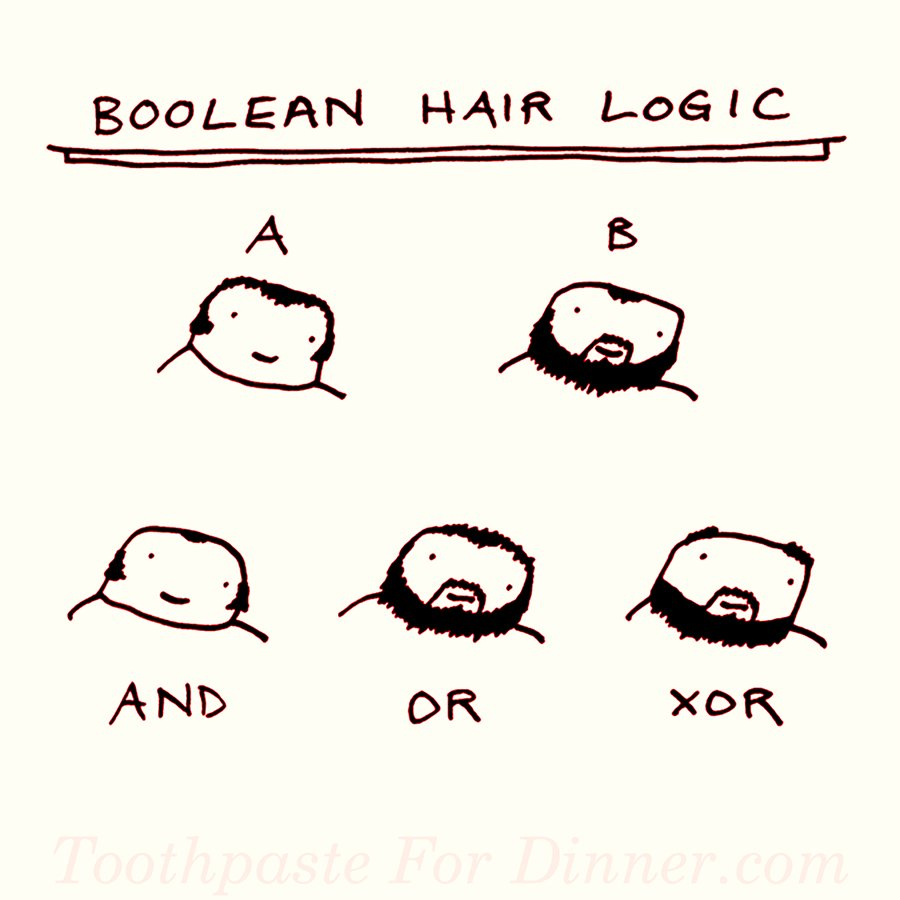
\includegraphics[width=0.8\textwidth]{boolean_hair_logic}
    \end{center}
\end{frame}

\begin{frame}{Negative gates}
	\pause
	\begin{center}
		$\OPnand, \OPnor, \OPxnor$ \par are the \textbf{negations} of \par $\OPand, \OPor, \OPxor$
	\end{center}
	\pause
	\begin{columns}
		\begin{column}{0.48\textwidth}
			\begin{center}
				\begin{align*}
					A \OPnand B &= \OPnot (A \OPand B) \\
					A \OPnor B &= \OPnot (A \OPor B) \\
					A \OPxnor B &= \OPnot (A \OPxor B)
				\end{align*}
			\end{center}
		\end{column}
		\pause
		\begin{column}{0.48\textwidth}
			\begin{center}
				\begin{circuitikz} \draw[color=\circuitcolour]
					(0,0) node[nand port] (gate) {}
					(gate.in 1) node[anchor=east] {$A$}
					(gate.in 2) node[anchor=east] {$B$}
					(gate.out)  node[anchor=west] {$A \OPnand B$}
					;
				\end{circuitikz}
				\begin{circuitikz} \draw[color=\circuitcolour]
					(0,0) node[nor port] (gate) {}
					(gate.in 1) node[anchor=east] {$A$}
					(gate.in 2) node[anchor=east] {$B$}
					(gate.out)  node[anchor=west] {$A \OPnor B$}
					;
				\end{circuitikz}
				\begin{circuitikz} \draw[color=\circuitcolour]
					(0,0) node[xnor port] (gate) {}
					(gate.in 1) node[anchor=east] {$A$}
					(gate.in 2) node[anchor=east] {$B$}
					(gate.out)  node[anchor=west] {$A \OPxnor B$}
					;
				\end{circuitikz}
			\end{center}
		\end{column}
	\end{columns}
\end{frame}

\begin{frame}{Any logic gate can be constructed from NAND gates}
    \begin{center}
        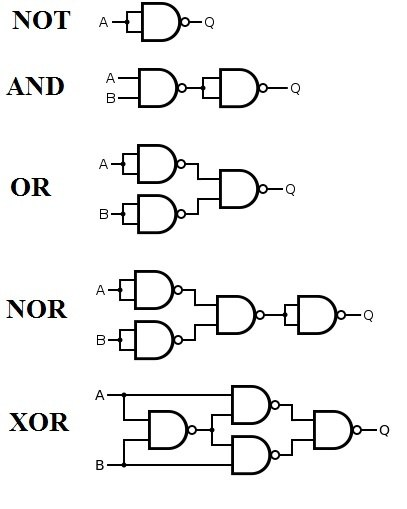
\includegraphics[height=0.7\textheight]{nand_gates}
    \end{center}
\end{frame}

\begin{frame}{What does this circuit do?}
	\centering
	\begin{circuitikz} \draw[color=\circuitcolour]
		(0,0) node[nand port] (gateA) {}
		(0,-2) node[nand port] (gateB) {}
		(gateA.out) -- ($ (gateA.out) + (0, -0.5) $) -- ($ (gateB.in 1) + (0, 0.5) $) -- (gateB.in 1) {}
		(gateB.out) -- ($ (gateB.out) + (0, 0.5) $) -- ($ (gateA.in 2) + (0, -0.5) $) -- (gateA.in 2) {}
		(gateA.out) -- ($ (gateA.out) + (0.5, 0) $) node[anchor=west] {$Q$}
		(gateB.out) -- ($ (gateB.out) + (0.5, 0) $) node[anchor=west] {$\overline{Q}$}
		(gateA.in 1) -- ($ (gateA.in 1) + (-0.5, 0) $) node[anchor=east] {$S$}
		(gateB.in 2) -- ($ (gateB.in 2) + (-0.5, 0) $) node[anchor=east] {$R$}
		;
	\end{circuitikz}
	\begin{itemize}
		\pause\item This is called a \textbf{NAND latch}
		\pause\item It ``remembers'' a single boolean value
		\pause\item Put a few billion of these together
			(along with some control circuitry)
			and you've got \textbf{memory}!
	\end{itemize}
\end{frame}

\begin{frame}{NAND gates}
    \begin{itemize}
        \pause\item All arithmetic and logic operations, as well as memory, can be built from NAND gates
        \pause\item So an entire computer can be built just from NAND gates!
        \pause\item Play the game: \url{http://nandgame.com}
        \pause\item NAND gate circuits are \textbf{Turing complete}
        \pause\item The same is true of NOR gates
    \end{itemize}
\end{frame}

